\newpage
\hypertarget{rules vis}{}
\subsection{Visual Rules}
\visHeader

\begin{enumerate}
\item[$\blacktriangleright$] In EA, open the diagram in the \texttt{Rules} package of your TGG project, automatically generated when you first created the TGG
project. As you can assume, this is where \emph{all} our rules will be contained.

\vspace{0.5cm}

\item[$\blacktriangleright$] Either hold \texttt{ctrl} and click, or via drag-and-drop from the TGG toolbox and create a new \texttt{Rule}
(Fig.~\ref{fig:create_tgg_rule}). Hold \texttt{Alt}, then press \texttt{enter} to raise its \texttt{Properties} dialogue. Set its name to
\texttt{BoxToDictionaryRule}.

\vspace{0.5cm}

\begin{figure}[htbp]
\begin{center}
  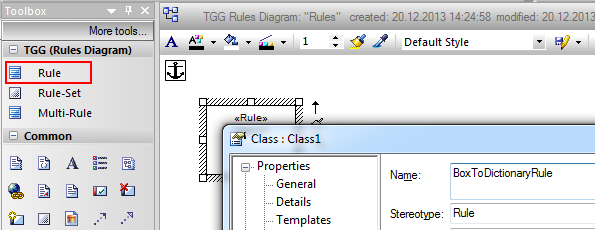
\includegraphics[width=\textwidth]{ea_TGGNewRule}
  \caption{Creating a TGG rule}
  \label{fig:create_tgg_rule}
\end{center}
\end{figure}

\item[$\blacktriangleright$] Now either select the rule and press \texttt{F10}, or right-click and go to ``Features \& Properties/Operations\ldots'' and create
a new void method called \texttt{BoxToDictionaryRule}.

\vspace{0.5cm}

\item[$\blacktriangleright$] Double click the rule to open its diagram. Hold \texttt{ctrl} again and drag-and-drop a \texttt{Box} from the project browser,
this as an instance of \texttt{Box}. Enter \texttt{box} as its name with \texttt{Create} as binding operator. Repeat to create an instance of
\texttt{Dictionary}.

\vspace{0.5cm}

\item[$\blacktriangleright$] Use quick-link to create a TGG Correspondence link between the elements from \texttt{box} to  \texttt{dictionary}, naming it
\texttt{boxToDictionary}. Be sure to select \texttt{Create New Link} in the dialogue that appears (Fig. \ref{fig:create_tgg_correspondence_link}). 

\newpage

\begin{figure}[htbp]
\begin{center}
  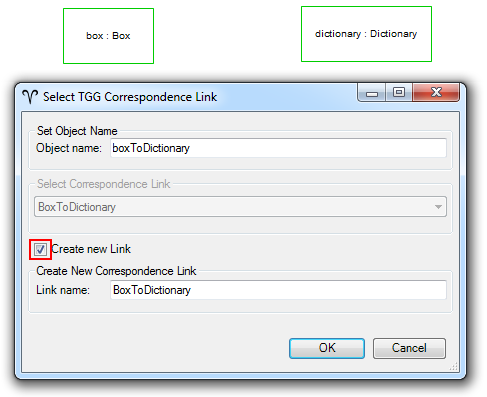
\includegraphics[width=0.8\textwidth]{ea_TGGBoxDictLink}
  \caption{Creating a TGG correspondence link via Quick-Link}
  \label{fig:create_tgg_correspondence_link}
\end{center}
\end{figure}

\end{enumerate}

Our current rule now creates a box, a dictionary, and an appropriate correspondence, all at the same time! What if we wanted to also connect the \texttt{name}
of the box to the \texttt{title} of the dictionary? We once again use \emph{attribute constraints}\footnote{First defined in Part III}! Attribute constraints
in TGG rules provide a bidirectional and high-level solution for attribute manipulation. Here we need a constraint which ensures that \texttt{box.name}
and \texttt{dictionary.title} are set to the same value.

\begin{enumerate}
  \item[$\blacktriangleright$] Nearly identical to how you created a \texttt{rule}, to create a constraint, either hold \texttt{ctrl} and click in
  the diagram (Fig.~\ref{fig:common_toolbox}), or drag-and-drop a \emph{TGG Constraint} from the \texttt{TGGRuleTolboxPage}.

\vspace{0.5cm}

\item[$\blacktriangleright$] Double click the constraint element to open its \texttt{TGGConstraint Dialog}, and choose \texttt{eq} (representing
\texttt{.equals}) under \texttt{Constraints}. Enter the values depicted in Fig.~\ref{fig:first_tgg_constraint} and officially add the constraint. Affirm with
\texttt{OK}.

\vspace{0.5cm}

\item[$\blacktriangleright$] Your rule should now resemble Fig.~\ref{fig:tgg_rule_with_constraint}, where the new links represent the dependencies between the
  constrain and objects involved

\newpage 

\begin{figure}[htbp]
\begin{center}
  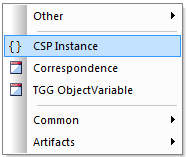
\includegraphics[width=0.3\textwidth]{ea_createTGGConstraint}
  \caption{Constraint from the Toolbox in EA}
  \label{fig:common_toolbox}
\end{center}
\end{figure}

\vspace{0.5cm}

\begin{figure}[htbp]
\begin{center}
  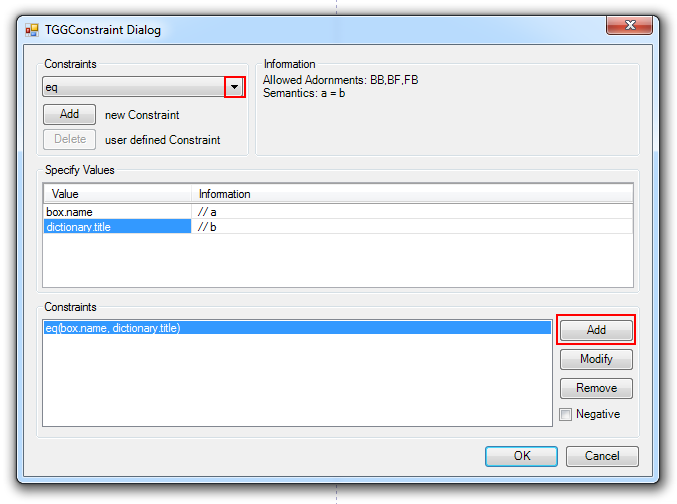
\includegraphics[width=0.7\textwidth]{ea_TGGConstraintDialog}
  \caption{Creating a Constraint in EA}
  \label{fig:first_tgg_constraint}
\end{center}
\end{figure}

\vspace{0.5cm}

\begin{figure}[h!]
\begin{center}
  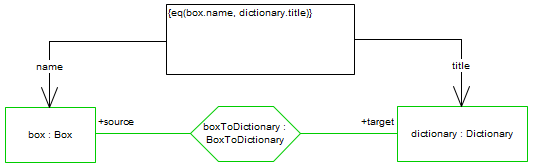
\includegraphics[width=\textwidth]{ea_TGGconstraintDependency}
  \caption{A TGG Rule with a Constraint}
  \label{fig:tgg_rule_with_constraint}
  \end{center}
\end{figure}

\newpage

\item[$\blacktriangleright$] To complete our first TGG rule, we still need to create the initial structure of a learning box. In contrast to the rather simple
dictionary, where \texttt{Dictionary} is a direct container for \texttt{Entry} objects, we have to create a number of connected \texttt{Partitions} that hold
the \texttt{Cards} in the learning box. Create three \texttt{Partition} object variables. You should be able to just drag-and-drop them now, without holding
\texttt{ctrl}. Be sure to also quick-link all the appropriate links (\texttt{next}, \texttt{previous}, and \texttt{box} references), so that your TGG rule
diagram closely resembles Fig.~\ref{fig:boxtodictionaryrule_complete}.


\begin{figure}[htbp]
\begin{center}
  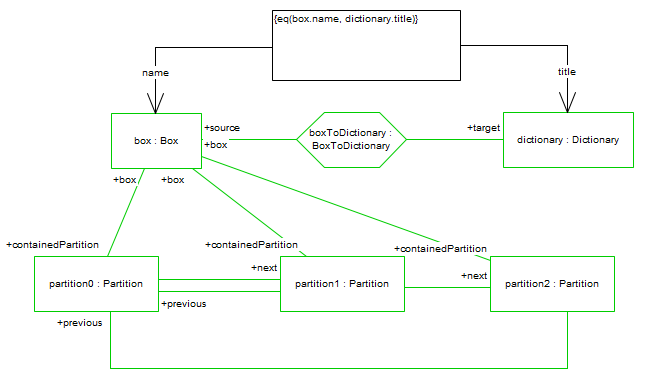
\includegraphics[width=\textwidth]{ea_TGGCompleteRule}
  \caption{Complete TGG rule diagram for \texttt{BoxToDictionaryRule}}
  \label{fig:boxtodictionaryrule_complete}
\end{center}
\end{figure}

\end{enumerate}

If you are in hurry, you can jump ahead and proceed to Section~\ref{sect:TGGs_in_Action}: TGGs in Action and transform a box to a dictionary and vice-versa, but
please be aware that your specified TGG (with just one rule) will only be able to cope with empty boxes and dictionaries. Handling additional elements
(i.e., cards in the learning box and entries in the dictionary) requires a second rule, which we will create next.

Do you remember one of our desired features of TGGs? Given one rule, we wanted to be able to create more relatively easily. So, to create our second rule to
take care of \texttt{card}s and \texttt{entry} objects from the Learning Box and Dictionary, we can use a cool, rule derivation feature provided by the editor.

\begin{enumerate}
  
\item[$\blacktriangleright$] First, confirm that your eMoflon control panel window is open (explain).
  
\item[$\blacktriangleright$] Simultaneously select \texttt{box}, \texttt{boxToDictionary}, \texttt{dictionary} and \texttt{partition0} in
\texttt{Box\-To\-Dictionary\-Rule} diagram by holding \texttt{ctrl} and selecting each one.
  
\item[$\blacktriangleright$] Switch to the \texttt{eMoflon TGG Functions} tab of the control panel, and press \texttt{Derive} as depicted in
Fig.~\ref{fig:derive_from_tgg_rule}. Enter  \texttt{CardToEntryRule} as the name in the dialog that pops up. The new TGG rule will be automatically derived, and
activate in a new window in the editor. 

\vspace{0.5cm}

\begin{figure}[htbp]
\begin{center}
 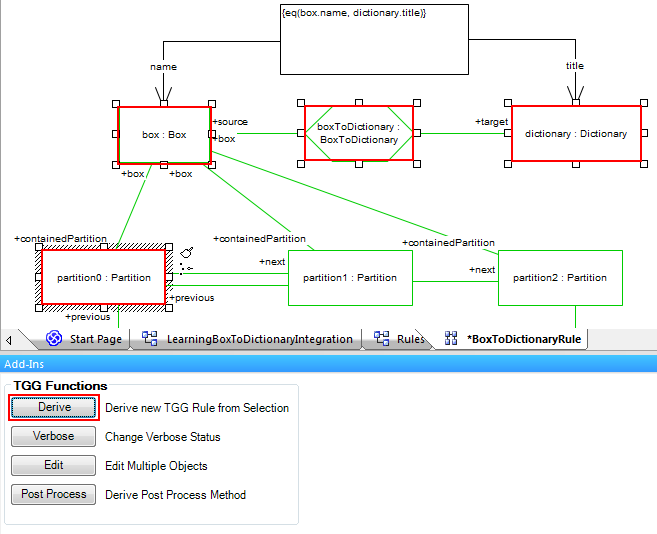
\includegraphics[width=\textwidth]{ea_selectPreDerivation}
  \caption{Derive from an existing TGG rule}
  \label{fig:derive_from_tgg_rule}
\end{center}
\end{figure}
\FloatBarrier

\item[$\blacktriangleright$] Add instances of \texttt{Card} and \texttt{Entry} to the rule and required links until the diagram closely resembles
Fig.~\ref{fig:cardtoentry_1}.

  \begin{figure}[htbp]
  \begin{center}
    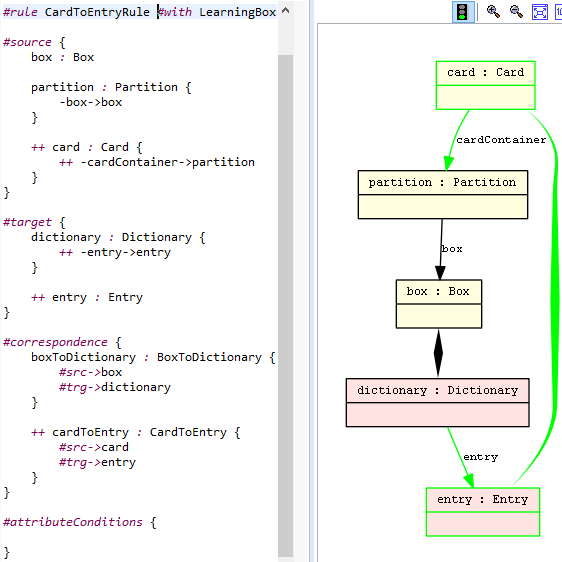
\includegraphics[width=\textwidth]{ea_cardToEntryRule}
    \caption{\texttt{CardToEntryRule} without attribute manipulation}
    \label{fig:cardtoentry_1}
  \end{center}
  \end{figure}

\end{enumerate}

As a final step, we now have to specify how attributes are to be handled via appropriate attribute constraints.

The \texttt{content} of an \texttt{Entry} in a \texttt{Dictionary} is to be of the form \texttt{<word>:<meaning>}, while the \texttt{face} of a \texttt{Card}
must read \texttt{Question:<word>}, and the \texttt{back} of the Card \texttt{Answer:<meaning>}.

Using two predefined attribute constraints, \texttt{addPrefix} and \texttt{concat}, we can specify this as a set of constraints:

\begin{enumerate}
 % Describe the dictionary class? Don't know reasoning behind these variables..
\item[$\blacktriangleright$] Double-click your constraint element and add an \texttt{addPrefix} constraint, where \texttt{prefix} is \texttt{``Question:''},
\texttt{a} is \texttt{word}, and \texttt{b} is \texttt{card.face}.
  
\item[$\blacktriangleright$] Create a second \texttt{addPrefix} constraint with \texttt{``Answer''}, \texttt{meaning}, \texttt{card.back}.

\item[$\blacktriangleright$] Finally, add a \texttt{concat} constraint, with \texttt{``~:~''} as the \texttt{separator}, and \texttt{word}, \texttt{meaning},
\texttt{entry.content} as \texttt{a}, \texttt{b}, \texttt{c}.

\item[$\blacktriangleright$] Your rule should now resemble Fig.~\ref{fig:cardtoentry_2}.

\begin{figure}[htbp]
\begin{center}
  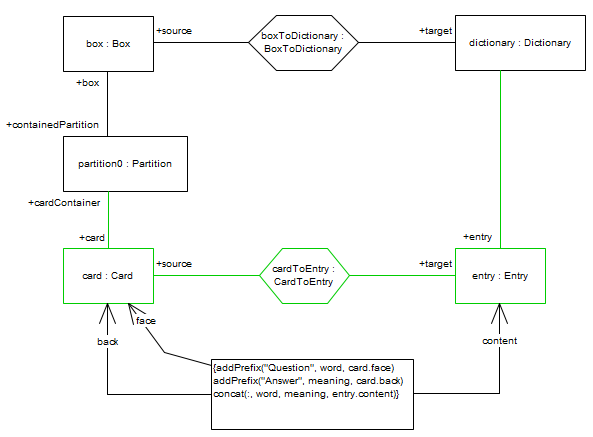
\includegraphics[width=\textwidth]{ea_completedCardToEntry}
  \caption{Attribute manipulation for \texttt{card} and \texttt{entry}}
  \label{fig:cardtoentry_2}
\end{center}
\end{figure}
\FloatBarrier
\end{enumerate}

% Rewrite to make this a bit more clear..
Finally, we have to specify how the partition (into which the new \texttt{card} is to be placed) must be chosen.
We shall implement the following rule: a card in a partition with index 0/1/2 corresponds to an \texttt{Entry} of level beginner/advanced/master.
This time, we must define a unique attribute constraint to handle this mapping. For now, we are just going to declare and use the attribute constraint, which
will be implemented later in Java.

\begin{enumerate}
\item[$\blacktriangleright$] Add one more constraint to your diagram. When you open the dialogue, don't choose a predefined constraint, but instead click
``Add'' below the dropdown menu. Enter the values given in Fig. \ref{fig:create_new_constraint}.

\vspace{0.5cm}

\begin{figure}[htbp]
\begin{center}
  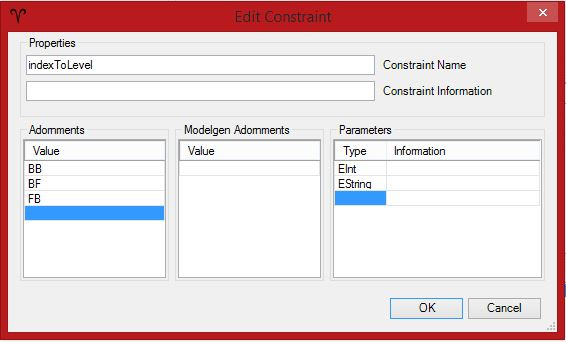
\includegraphics[width=\textwidth]{ea_uniqueConstraint}
  \caption{Create a user defined constraint.}
  \label{fig:create_new_constraint}
\end{center}
\end{figure}
\FloatBarrier

\item[$\blacktriangleright$] Saving this new constraint, then select it from the drop down menu and enter \texttt{partition0.index} as \texttt{Integer} and
\texttt{entry.level} as the \texttt{String}.
\end{enumerate}

After defining the dependencies of the constraint, your complete TGG rule should resemble Fig.~\ref{fig:cardtoentry_complete}.

\begin{figure}[htbp]
\begin{center}
  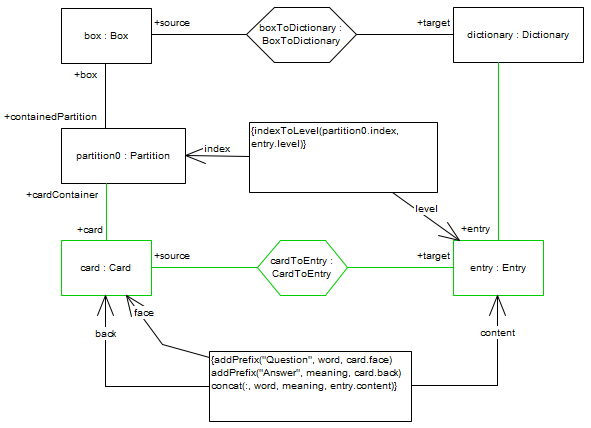
\includegraphics[width=\textwidth]{ea_finalCardToEntry}
  \caption{\texttt{CardToEntryRule} with complete attribute manipulation}
  \label{fig:cardtoentry_complete}
\end{center}
\end{figure}

Just like the patterns describing \emph{structural} correspondence,  attribute constraints can be automatically \emph{operationalized} as required for  concrete
transformations (forward, backward). Even more interesting, a set of constraints might have to be ordered a bit differently depending on the direction of the
transformation, and some constraints might have to be checked for already set attributes, while others must set values appropriately to fulfill the constraint.

For built-in or \emph{library} constraints such as \emph{eq}, \emph{addPrefix} and \emph{concat}, you do not need to worry about these details and can just
express what should hold -- everything else is handled automatically.

In many cases, however, a constraint might be very problem-specific, such as our \emph{indexToLevel} constraint, and there might not be any fitting combination
of library constraints to express the consistency condition.

In such a case, the new attribute constraint must be declared before its use.

The list of \emph{adornments} in the declaration specifies the cases for which the constraint can be operationalized. Each adornment consists of a \texttt{B}
for bound or an \texttt{F} for free, for each argument of the constraint. This is much simpler than its sounds so lets take a look at our example:

\begin{description}

\item[BB] means that the \texttt{partition.index} and \texttt{entry.level} can both be \emph{bound}, i.e., already have assigned values.
In this case, the \emph{operation} (the operationalized constraint) must check if the assigned values are correct.

\item[BF] means that \texttt{partition.index} is \emph{bound} and \texttt{entry.level} is \emph{free}, i.e., the operation must determine and assign the correct
value to \texttt{entry.level} using \texttt{partition.index}.

\item[FB] means that \texttt{partition.index} is \emph{free} and \texttt{entry.level} is \emph{bound}, i.e., the operation must determine and assign the correct
value to \texttt{parti\-tion.in\-dex} using \texttt{entry.level}.

\end{description}

Note that we decide not to support \textbf{FF} as we would have to generate a consistent pair of index and level.
Although this is possible and might even make sense for some applications, in our case it does not (the pair is not unique\ldots which pair should we take?).

At compile time, the set of constraints (also called \emph{Constraint Satisfaction Problem} (CSP)) for every TGG rule is ``solved'' for each case (forward,
backward) by operationalizing all constraints and determining a feasible (compatible to the declared adornments of each constraint) sequence in which the
operations can be executed. An exception is thrown if this is not possible.
